%%%%%%%%%%%%%%%%%%%%%%%%%%%%%%%%%%%%%%
% LaTeX poster template
% Created by Nathaniel Johnston
% August 2009
% http://www.nathanieljohnston.com/2009/08/latex-poster-template/
%%%%%%%%%%%%%%%%%%%%%%%%%%%%%%%%%%%%%%

\documentclass[final]{beamer}
\usepackage[scale=1.24]{beamerposter}
\usepackage{graphicx}			% allows us to import images
\usepackage{verbatim}

%-----------------------------------------------------------
% Define the column width and poster size
% To set effective sepwid, onecolwid and twocolwid values, first choose how many columns you want and how much separation you want between columns
% The separation I chose is 0.024 and I want 4 columns
% Then set onecolwid to be (1-(4+1)*0.024)/4 = 0.22
% Set twocolwid to be 2*onecolwid + sepwid = 0.464
%-----------------------------------------------------------

\newlength{\sepwid}
\newlength{\onecolwid}
\newlength{\twocolwid}
\newlength{\threecolwid}
\setlength{\paperwidth}{48in}
\setlength{\paperheight}{36in}
\setlength{\sepwid}{0.024\paperwidth}
\setlength{\onecolwid}{0.22\paperwidth}
\setlength{\twocolwid}{0.464\paperwidth}
\setlength{\threecolwid}{0.708\paperwidth}
\setlength{\topmargin}{-0.5in}
\usetheme{confposter}
\usepackage{exscale}

%-----------------------------------------------------------
% The next part fixes a problem with figure numbering. Thanks Nishan!
% When including a figure in your poster, be sure that the commands are typed in the following order:
% \begin{figure}
% \includegraphics[...]{...}
% \caption{...}
% \end{figure}
% That is, put the \caption after the \includegraphics
%-----------------------------------------------------------

\usecaptiontemplate{
\small
\structure{\insertcaptionname~\insertcaptionnumber:}
\insertcaption}

%-----------------------------------------------------------
% Define colours (see beamerthemeconfposter.sty to change these colour definitions)
%-----------------------------------------------------------

\setbeamercolor{block title}{fg=ngreen,bg=white}
\setbeamercolor{block body}{fg=black,bg=white}
\setbeamercolor{block alerted title}{fg=white,bg=dblue!70}
\setbeamercolor{block alerted body}{fg=black,bg=dblue!10}

%-----------------------------------------------------------
% Name and authors of poster/paper/research
%-----------------------------------------------------------

\title{Part Handling in qooxdoo 3}
\author{Thomas Herchenr\"oder}
\institute{1\&1 Internet AG}

%-----------------------------------------------------------
% Start the poster itself
%-----------------------------------------------------------

\begin{document}
\begin{frame}[t]
  \begin{columns}[t]												% the [t] option aligns the column's content at the top
    \begin{column}{\sepwid}\end{column}			% empty spacer column
    \begin{column}{\onecolwid}
      \begin{block}{Parts}
        \textit{Parts} are a means to \textit{logically} partition a qooxdoo
        application, so that those parts can be loaded \textit{incrementally}
        and \textit{on demand}. Parts are defined through
        configuration, and the \textit{Generator} 
        distributes class code and resource information across multiple script
        files that are then retrieved via HTTP. The aim is to avoid loading
        of unnecessary code and data into the browser.
      \end{block}
      \vskip2ex
      \begin{block}{Concepts}
        The Generator collects \textit{class} code into
        \textit{scripts} (.js files). Scripts are grouped into
        \textit{packages}. Scripts of the same package are always loaded
        together. Each \textit{part} is
        implemented by a collection of packages, each package might be required
        by multiple parts. qooxdoo's \textit{PartLoader} loads all packages for
        a part that has been required, but have not been loaded yet.
        \begin{figure}
          \begin{center}
            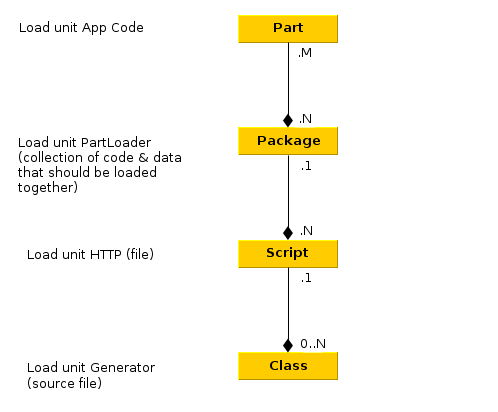
\includegraphics[width=10in]{g_relations.png} \\
            \caption{Relations between parts, packages, scripts and classes.}
            \label{fig:corrSubsys}
          \end{center}
        \end{figure}
      \end{block}


      \begin{block}{Configuring Parts}
        What to put in the \textit{include} key of the part definitions.
        "include list" means all entries after glob expansion.
        \begin{itemize}
          \item the \textit{boot} part should have the same include definition
            as the application
          \item include lists must be \textit{free of overlaps}
          \item \textit{load dependencies} of one part must not be in include lists of
            other parts
        \end{itemize}
      \end{block}

      \vskip2ex
    \end{column}

    % column 2

    \begin{column}{\sepwid}\end{column}			% empty spacer column

    \begin{column}{\twocolwid}  % 2-column middle
    \begin{columns}[t,totalwidth=\twocolwid] % split in 2
    \begin{column}{\onecolwid}
      \begin{block}{}
        \begin{itemize}
          \item don't define include lists along \textit{physically boundaries} (name
            spaces, libraries, ...)
          \item don't define parts with \textit{framework classes}
        \end{itemize}
        Some of these criteria a checked by the Generator.
      \end{block}

      \begin{block}{2-Phase Package Calculation}
        Assign classes to packages in a 2-step process:
        \begin{itemize}
          \item \textbf{equivalence sets} group all classes that are required by the
            same set of parts
          \item \textbf{merging} (or collapsing) resolve smaller packages into
            larger ones
        \end{itemize}
      \end{block}
    \end{column}

    \begin{column}{\sepwid}\end{column}			% empty spacer column
    \begin{column}{\onecolwid}
      \begin{block}{Equivalence sets}
        To construct the equivalence sets for the classes:
        \begin{itemize}\justifying
          \item calculate the class list for each part (starting from the
            part's \textit{include} config)
          \item assigne each class the parts which require it
          \item group classes that are required by the same parts
        \end{itemize}
        If $N$ is the number of defined parts then\\
        \begin{center}
          $ max(count(equivalence\_sets(N))) = 2^{N} - 1 $
        \end{center}
      \end{block}
    \end{column}

    \end{columns}

    % center image

    \begin{figure}   % ACTUAL two-column-wide column
      \begin{center}
        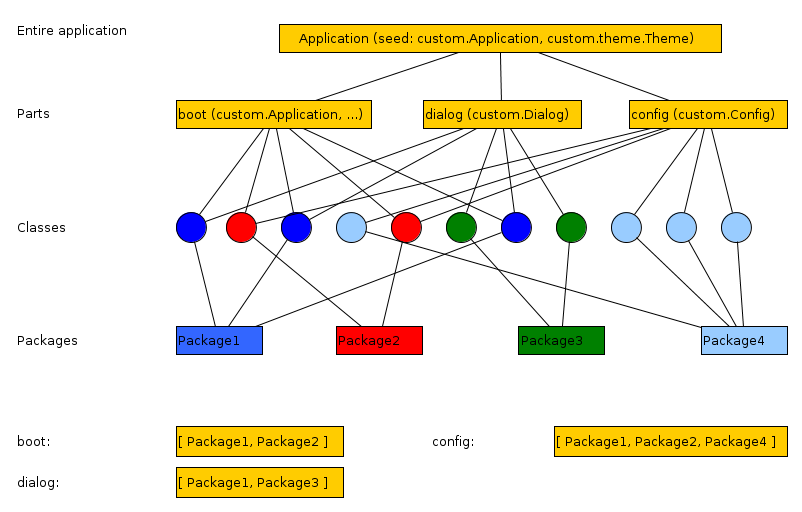
\includegraphics[width=20in]{g_part_layers.png} \\
        \caption{Mapping parts to classes, and classes to packages.}
        \label{fig:corrSubsys}
      \end{center}
    \end{figure}

    % middle bottom

    \begin{columns}[t,totalwidth=\twocolwid]
    \begin{column}{\onecolwid}
      \begin{block}{Part Assertions}
        \begin{itemize}
          \item parts are \textbf{lazy run deps}
          \item each part is \textbf{self-contained} \textit{wrt} load deps 
          \item this is also true for \textit{collapsePartsByOrder}, parts
            can be loaded out-of-order
          \item every class is only loaded \textbf{once}
          \item classes are \textbf{load-ordered} within a package, packages are
            load-ordered within a part
        \end{itemize}
      \end{block}

    \end{column}

    \begin{column}{\onecolwid}
      \begin{block}{References}
        \small{\begin{thebibliography}{99}
          \bibitem P``Parts and Packages Overview'', qooxdoo Manual, http://bit.ly/1hL6cqU
          \bibitem U``Using Parts'', qooxdoo Manual, http://bit.ly/17y8MMH
          \bibitem G``Generator Config Keys - packages'', qooxdoo Manual, http://bit.ly/177sNXW 
          \bibitem qqx.io.PartLoader, qooxdoo API, http://bit.ly/1cvQM2Q 
        \end{thebibliography}}
      \end{block}

    \end{column}

    \end{columns}
    \end{column}  % 2-column middle

    % column 4

    \begin{column}{\sepwid}\end{column}			% empty spacer column

    \begin{column}{\onecolwid}

      \begin{block}{Package Dependencies}
        If classes $c1, c2$ and packages $p1, p2$, then\\
        \begin{center}
          $if\ c1 \in p1\ and\ c2 \in p2\ and\ depends(c1,c2) \Rightarrow
          depends(p1,p2)$
        \end{center}
      \end{block}

      \begin{block}{Package Merging}
        Classes from the yielding package are added to the receiving package.
        The yielding package is removed. 
        Let $p1$ be a package for merging into $p2$, $P(x)$ be
        the set of parts a package is used in, $Deps(x)$ be the depedencies of
        a class or package, then
        \begin{itemize}
          \item $P(p1) \subset P(p2)$  [$p2$ must at least be used where $p1$ is
            used]
          \item after the merge: $for\_each\_class\ c \in p1: Deps(c) \subset p1\ and\ 
            ordered(p1)$
          \item $replace(p1, p2)\ in\ all\ P(p1)$ [use $p2$ in all parts where $p1$ was
            used]
        \end{itemize}
        This is done with \textit{names}, no code is shuffled around.
        Merging can be more aggressive if \textit{collapsePartsByOrder} is given
        in config.

        Package calculation log (Feedreader):

        \tiny\begin{verbatim}
          >>> Creating part structures...
            - Part \#addfeed => 1
            - Part \#boot => 2
            - Part \#settings => 4

          >>> Assembling parts
            - part addfeed  
            - Part \#addfeed depends on 245 classes
            - part boot  
            - Part \#boot depends on 364 classes
            - part settings  
            - Part \#settings depends on 274 classes

          >>> Package summary : 6 packages
            - Package \#7 contains 228 classes
            - [<Class:qx.module.Animation>, <Class:qx.ui.layout.Atom>, <Class:qx.bom.clien
            - Package \#7 depends on these packages: []
            - Package \#6 contains 23 classes
            - [<Class:qx.io.PartLoader>, <Class:qx.bom.request.Script>, <Class:qx.io.part.
            - Package \#6 depends on these packages: ['7']
            - Package \#5 contains 4 classes
            - [<Class:qx.ui.form.IColorForm>, <Class:qx.ui.form.Resetter>, <Class:qx.ui.fo
            - Package \#5 depends on these packages: ['7']
            - Package \#4 contains 19 classes
            - [<Class:qx.ui.form.RadioGroup>, <Class:qx.ui.form.RadioButton>, <Class:qx.th
            - Package \#4 depends on these packages: ['5', '6', '7']
            - Package \#2 contains 113 classes
            - [<Class:qx.ui.splitpane.Pane>, <Class:qx.ui.toolbar.Part>, <Class:qx.theme.I
            - Package \#2 depends on these packages: ['6', '7']
            - Package \#1 contains 13 classes
            - [<Class:qx.ui.form.renderer.IFormRenderer>, <Class:qx.util.Validate>, <Class
            - Package \#1 depends on these packages: ['7']

          >>> Part summary : 3 parts
            - Part \#addfeed packages(3): \#7, \#5, \#1
            - Part \#boot packages(3): \#7, \#6, \#2
            - Part \#settings packages(4): \#7, \#5, \#6, \#4

            - Total of packages used in parts: 10

          >>> Collapsing parts  

          >>> Collapsing parts by collapse order...
            - Collapse group 0 [u'boot']
              - collapsing unique packages...
                - Search a target package for package \#2
                  - Merge package \#2 into \#6
                    - Adding packages dependencies to target package: ['7']
                    - Target package \#6 now depends on: ['7']
                - Search a target package for package \#6
                  - Merge package \#6 into \#7
                    - Adding packages dependencies to target package: []
                    - Target package \#7 now depends on: []
                - Search a target package for package \#7
                - Search a target package for package \#7
              - collapsing common packages...
                - Search a target package for package \#7

          >>> Collapsing parts by package sizes...
            - Minimum size: 10KB
              - Package \#4: 210KB
              - Package \#1: 102KB
              - Package \#5: 12KB
              - Package \#7: 3266KB

          >>> Package summary : 4 packages
            - Package \#7 contains 364 classes
            - [<Class:qx.module.Animation>, <Class:qx.ui.layout.Atom>, <Class:qx.bom.clien
            - Package \#7 depends on these packages: []
            - Package \#5 contains 4 classes
            - [<Class:qx.ui.form.IColorForm>, <Class:qx.ui.form.Resetter>, <Class:qx.ui.fo
            - Package \#5 depends on these packages: ['7']
            - Package \#4 contains 19 classes
            - [<Class:qx.ui.form.RadioGroup>, <Class:qx.ui.form.RadioButton>, <Class:qx.th
            - Package \#4 depends on these packages: ['5', '7']
            - Package \#1 contains 13 classes
            - [<Class:qx.ui.form.renderer.IFormRenderer>, <Class:qx.util.Validate>, <Class
            - Package \#1 depends on these packages: ['7']

          >>> Part summary : 3 parts
            - Part \#addfeed packages(3): \#7, \#5, \#1
            - Part \#boot packages(1): \#7
            - Part \#settings packages(3): \#7, \#5, \#4

            - Total of packages used in parts: 7

          >>> Verifying parts  
            - Verifying packages-to-parts relations...
            - Verifying individual parts...
            - Part: addfeed
            - Part: boot
            - Part: settings
        \end{verbatim}

        \vspace{0.75in}
        \begin{center}
          
\includegraphics[width=2in]{qx.png}
        \end{center}
      \end{block}

    \end{column}

  \end{columns}
\end{frame}
\end{document}
